
\begin{frame}
\frametitle{Clay GDSM Sensitivity Analysis}
\footnotesize{
\begin{itemize}
\item Barrier Degradation
\item Sorption
\item Solubility
\item Advective Velocity
\item Diffusivity
\end{itemize}
\begin{figure}[htbp!]
  \begin{center}
    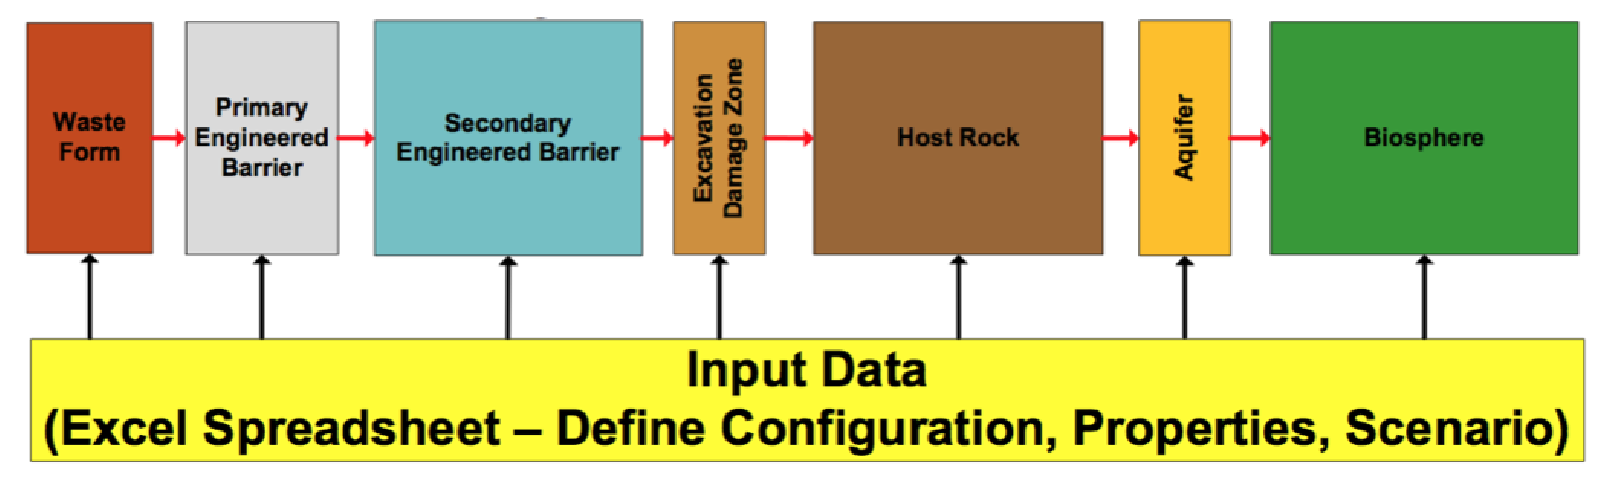
\includegraphics[width=0.7\textwidth]{./images/clay_gdsm.eps}
  \end{center}
  \caption{The Clay Generic Disposal System Model (GDSM) was used for 
  preliminary sensitivity analysis, abstraction iteration, and validation.
  This figure was reproduced from Figure 3.3-2 in \cite{clayton_generic_2011}.}
  \label{fig:clay_gdsm}
\end{figure}

}
\end{frame}

\begin{frame}
  \frametitle{Nested Components}
  The NuclideModel in a Component can be interchangeably represented by any of 
  the four nuclide transport models. 
    \begin{itemize}
      \item Degradation Rate Based Failure Model
      \item Mixed Cell with Degradation, Sorption, Solubility Limitation
      \item Lumped Parameter Model
      \item 1 Dimensional Approximate Advection Dispersion Solution, Brenner 
      \cite{brenner_diffusion_1962}
    \end{itemize}
\end{frame}



%\begin{frame}
%  \frametitle{Component Interfaces}
%  \footnotesize{
%Solutions to this equation can be categorized by their boundary conditions and 
%those boundary conditions serve as the interfaces between components in the 
%Cyder library of nuclide transport models.
%
%  \begin{figure}[htp!]
%    \begin{center}
%      \def\svgwidth{\textwidth}
%      \input{images/flow.eps_tex}
%    \end{center}
%    \caption{The boundaries between components are robust interfaces defined by 
%    Source Term, Dirichlet, Neumann, and Cauchy boundary conditions.}
%    \label{fig:flow}
%  \end{figure}
%  }
%\end{frame}

\begin{frame}
  \frametitle{Radionuclide Transport: Degradation Rate Based Release}
  \begin{figure}[h!]
  \begin{center}
    \def\svgwidth{.7\textwidth}
    \begin{figure}[h!]
  \begin{center}
    \def\svgwidth{.7\textwidth}
    \begin{figure}[h!]
  \begin{center}
    \def\svgwidth{.7\textwidth}
    \input{./images/deg_volumes.eps_tex}
  \end{center}
  \caption[Constituents of a Degradation Rate Control Volume]{The control volume contains an 
  intact volume $V_i$ and a degraded volume, $V_d$. Contaminants in $V_d$ are 
  available for transport, while contaminants in $V_i$ are contained.}
  \label{fig:deg_volumes}
\end{figure}


  \end{center}
  \caption[Constituents of a Degradation Rate Control Volume]{The control volume contains an 
  intact volume $V_i$ and a degraded volume, $V_d$. Contaminants in $V_d$ are 
  available for transport, while contaminants in $V_i$ are contained.}
  \label{fig:deg_volumes}
\end{figure}


  \end{center}
  \caption[Constituents of a Degradation Rate Control Volume]{The control volume contains an 
  intact volume $V_i$ and a degraded volume, $V_d$. Contaminants in $V_d$ are 
  available for transport, while contaminants in $V_i$ are contained.}
  \label{fig:deg_volumes}
\end{figure}


\end{frame}



\begin{frame}
  \frametitle{Radionuclide Transport : Mixed Cell with Sorption and Solubility}
  \begin{figure}[h!]
  \begin{center}
    \def\svgwidth{\textwidth}
    \begin{figure}[h!]
  \begin{center}
    \def\svgwidth{\textwidth}
    \begin{figure}[h!]
  \begin{center}
    \def\svgwidth{\textwidth}
    \input{./images/deg_sorb_volumes.eps_tex}
  \end{center}
  \caption[Constituents of a Mixed Cell Control Volume]{The degraded volume is 
  modeled as a solid degraded volume, $V_{ds}$, and a fluid degraded volume, 
  $V_{df}$. The intact volume is modeled as an intact solid volume, $V_{is}$, and 
  an intact fluid volume $V_{if}$.  Only contaminants in $V_{df}$ are available 
  for transport.}
  \label{fig:deg_sorb_volumes}
\end{figure}


  \end{center}
  \caption[Constituents of a Mixed Cell Control Volume]{The degraded volume is 
  modeled as a solid degraded volume, $V_{ds}$, and a fluid degraded volume, 
  $V_{df}$. The intact volume is modeled as an intact solid volume, $V_{is}$, and 
  an intact fluid volume $V_{if}$.  Only contaminants in $V_{df}$ are available 
  for transport.}
  \label{fig:deg_sorb_volumes}
\end{figure}


  \end{center}
  \caption[Constituents of a Mixed Cell Control Volume]{The degraded volume is 
  modeled as a solid degraded volume, $V_{ds}$, and a fluid degraded volume, 
  $V_{df}$. The intact volume is modeled as an intact solid volume, $V_{is}$, and 
  an intact fluid volume $V_{if}$.  Only contaminants in $V_{df}$ are available 
  for transport.}
  \label{fig:deg_sorb_volumes}
\end{figure}


\end{frame}

\begin{frame}
  \frametitle{Radionuclide Transport : Mixed Cell Sorption}
The mass of contaminant sorbed into the degraded and precipitated solids can be
found using a linear isotherm model \cite{schwartz_fundamentals_2004},
characterized by the relationship 
\begin{align}
s_{i} &= K_{di} C_{i}
\label{linear_iso}
\intertext{where}
s_i &= \mbox{ the solid concentration of isotope i }[kg/kg]\nonumber\\
K_{di} &= \mbox{ the distribution coefficient of isotope i}[m^3/kg]\nonumber\\
C_i &= \mbox{ the liquid concentration of isotope i }[kg/m^3].\nonumber
\end{align}
\end{frame}


\begin{frame}
  \frametitle{Radionuclide Transport : Mixed Cell Solubility Limitation}
In addition to engineered barriers, contaminant transport is constrained by 
  the solubility limit \cite{hedin_integrated_2002}, 
    \begin{align}
      m_{s,i} &\leq V_w C_{sol,i},
    \intertext{where}
      m_{s,i} &= \mbox{ solubility limited mass of isotope i in volume }V_w [kg]\nonumber\\ 
      V_w &= \mbox{ volume of the solution }[m^3]\nonumber\\
      C_{sol,i} &= \mbox{ solubility limit, the maximum concentration of i }[kg/m^3].\nonumber
    \end{align}
\end{frame}


\begin{frame}
  \frametitle{Radionuclide Transport: Lumped Parameter Transport Model}
\footnotesize{
\begin{figure}[htbp!]
  \begin{center}
    \def\svgwidth{\textwidth}
    \input{images/lumpedseries.eps_tex}
  \end{center}
  \caption{ The method by which each lumped parameter component is modeled is
according to a relationship between the incoming concentration, $C_{in}(t)$,
and the outgoing concentration, $C_{out}(t)$.}
  \label{fig:lumpedseries}
\end{figure}

\begin{align}
  C_{out}(t) &= \int_0^\infty C_{in}(t-t')g(t')e^{-\lambda t'}dt'
  \label{lumped2}
  \intertext{where}
  t'  &= \mbox{ time of entry }[s]\nonumber\\
  t-t'  &= \mbox{ transit time }[s]\nonumber\\
  g(t-t')  &= \mbox{ response function, a.k.a. transit time distribution}[-]\nonumber\\
  \lambda &= \mbox{ radioactive decay constant}[s^{-1}].\nonumber
\end{align}
}
\end{frame}

\begin{frame}
  \frametitle{Radionuclide Transport: 1D Finite, Cauchy B.C.}
\begin{figure}[htbp!]
  \begin{center}
    \def\svgwidth{.5\textwidth}
    \input{images/1dfin.eps_tex}
  \end{center}
  \caption{A one dimensional, finite, unidirectional flow,
  solution with Cauchy and Neumann boundary conditions 
\cite{van_genuchten_analytical_1982, brenner_diffusion_1962}.}
  \label{fig:1dinf}
\end{figure}
\end{frame}


\begin{frame}[ctb!]
\frametitle{Clay GDSM Degradation Rate Sensitivity}

\begin{figure}[ht!]
\centering
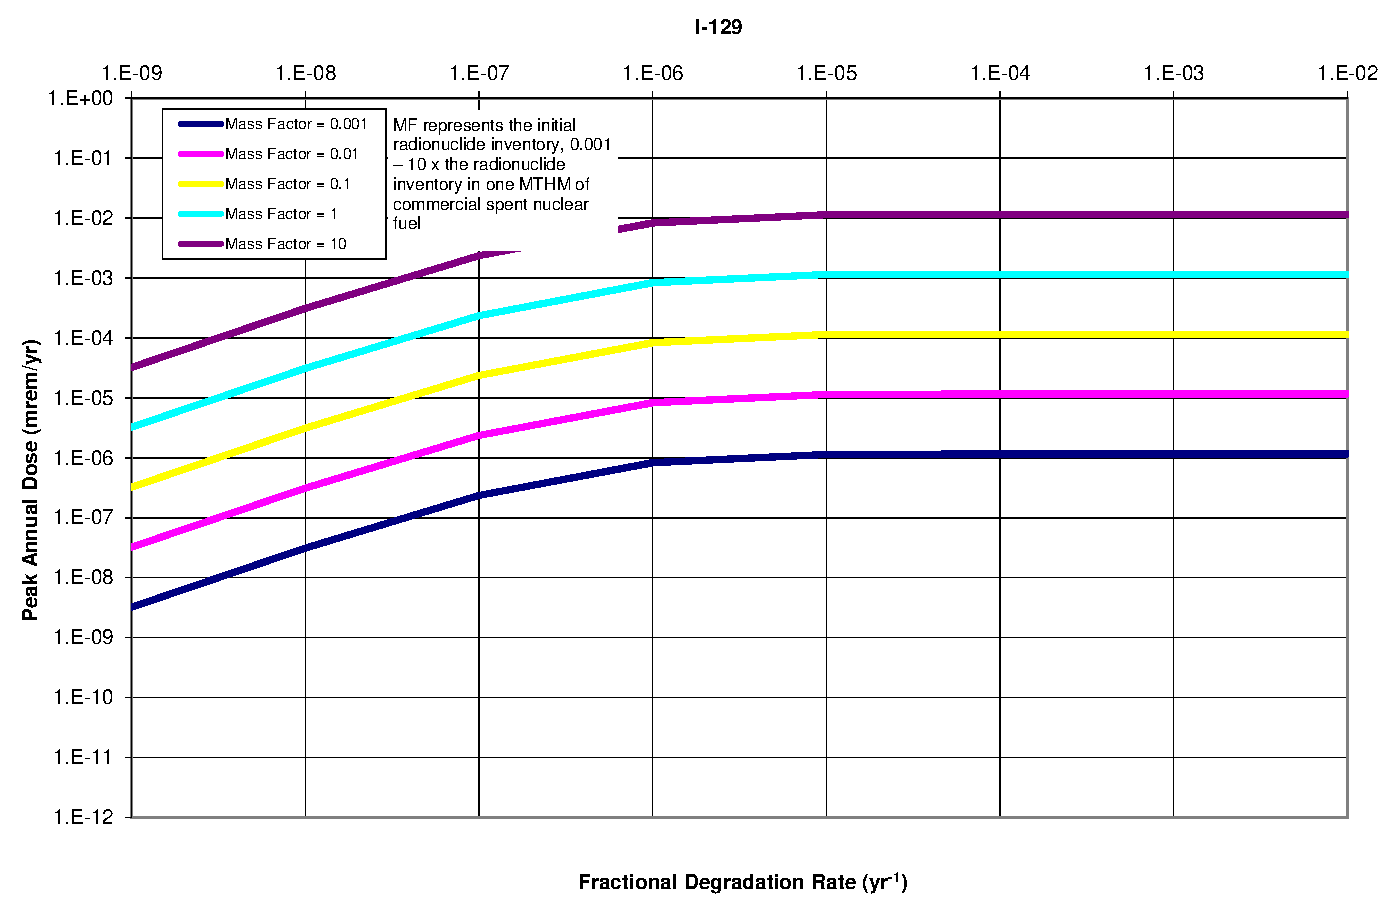
\includegraphics[width=0.6\textwidth]{./nuclide_demonstration/DegRate/I-129.eps}
\caption{$^{129}I$ waste form degradation rate sensitivity.}
\label{fig:WFDegI129}
\end{figure}
\end{frame}

\begin{frame}[ctb]
\frametitle{Cyder Degradation Rate Sensitivity}

\begin{figure}[htbp!]
\begin{center}
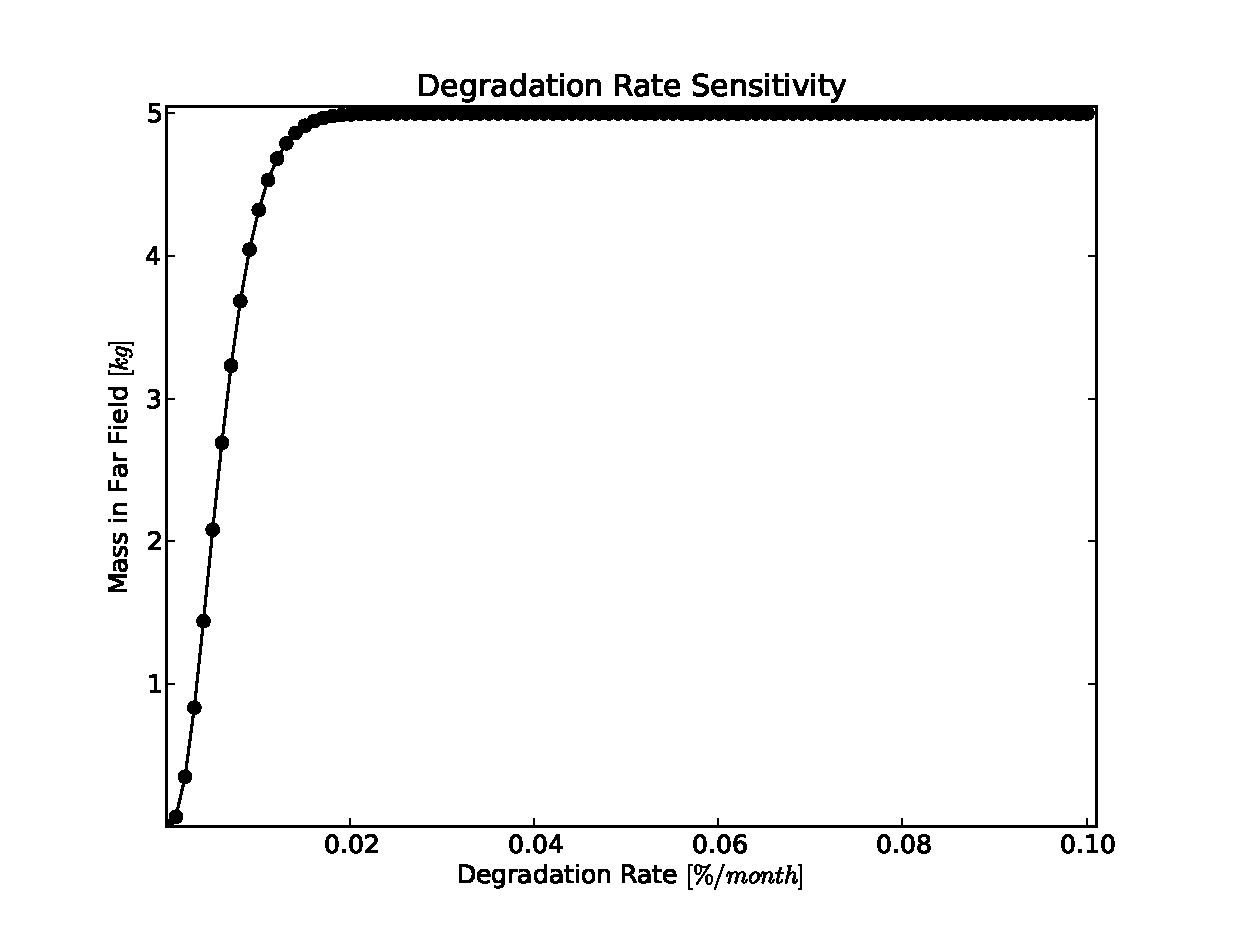
\includegraphics[width=0.7\linewidth]{./nuclide_demonstration/deg.eps}
\end{center}
\caption{Sensitivity demonstration of the degradation rate in \Cyder for an 
arbitrary isotope.}
\label{fig:deg}
\end{figure}
\end{frame}




\subsubsection{Reference Sorption Coefficient Sensitivity}

In the parametric sensitivity analysis discussed in Section \ref{sec:sorption}, 
the expected inverse relationship between the retardation factor and resulting 
peak annual dose was found for all elements that were not assumed to be 
effectively infinitely soluble. In the low retardation coefficient cases, a 
regime is established in which the peak annual dose is entirely unaffected by 
changes in retardation coefficient. For large values of retardation 
coefficient, the sensitivity to small changes in the retardation coefficient 
increases dramatically. In that sensitive regime, the change in peak annual 
dose is inversely related to the retardation coefficient. Between these two 
regimes was a transition regime, in which the $K_d$ factor ranges from 
$1\times10^{-5}$ to $5\times10^{0} [-]$.

It is clear from Figures \ref{fig:KdSumFactor} and \ref{fig:KdSum} that 
for retardation coefficients greater than a threshold, the 
relationship between peak annual dose and retardation coefficient is a strong 
inverse one. 

\begin{figure}[ht]
\centering
\includegraphics[width=0.7\linewidth]{./chapters/nuclide_sensitivity/clay/Sorption/Retardation_Summary_kdFactor.eps}
\caption{$K_d$ factor sensitivity.  The peak annual dose due to an inventory, 
$N$, of each isotope.}
\label{fig:KdSumFactor}
\end{figure}

\begin{figure}[ht]
\centering
\includegraphics[width=0.7\linewidth]{./chapters/nuclide_sensitivity/clay/Sorption/Retardation_Summary_kd.eps}
\caption{$K_d$ sensitivity.  The peak annual dose due to an inventory, 
$N$, of each isotope.}
\label{fig:KdSum}
\end{figure}

\FloatBarrier


\subsubsection{Reference Sorption Coefficient Sensitivity}

In the parametric analysis of \Cyder performance, it was shown that sorption 
sensitivity behavior closely matched that of the \gls{GDSM} sensitivity 
behaviors. Specifically, in Figure \ref{fig:kd_result}, increasing the retardation 
coefficient results in a smooth but dramatic turnover. 

\begin{figure}[ht]
\centering
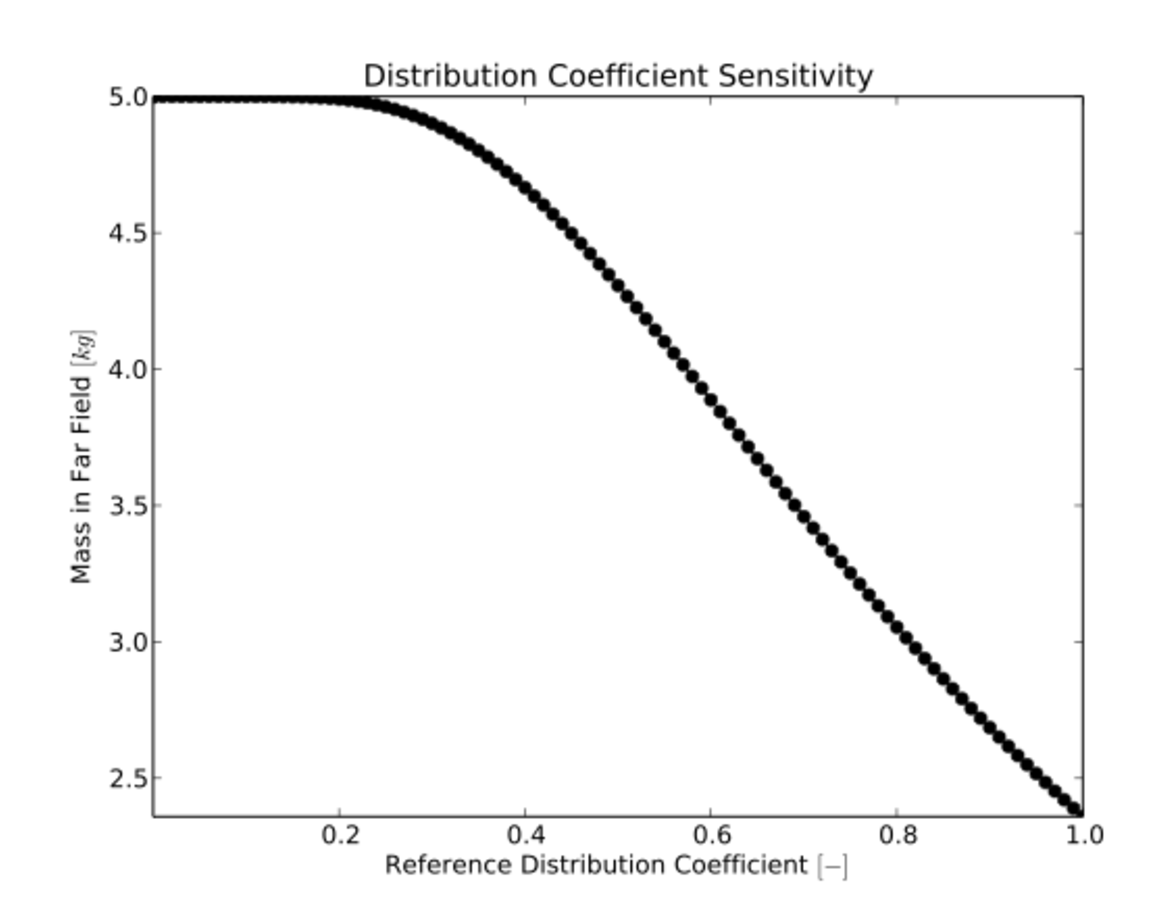
\includegraphics[width=0.7\linewidth]{./chapters/demonstration/bench/kd.eps}
\caption{$K_d$ factor sensitivity in the \Cyder tool for an arbitrary isotope 
assigned a variable $K_d$ coefficient.} 
\label{fig:kd_result}
\end{figure}


\begin{frame}[ctb!]
\frametitle{Clay GDSM Solubility Sensitivity}
\begin{figure}[htb!]
\centering
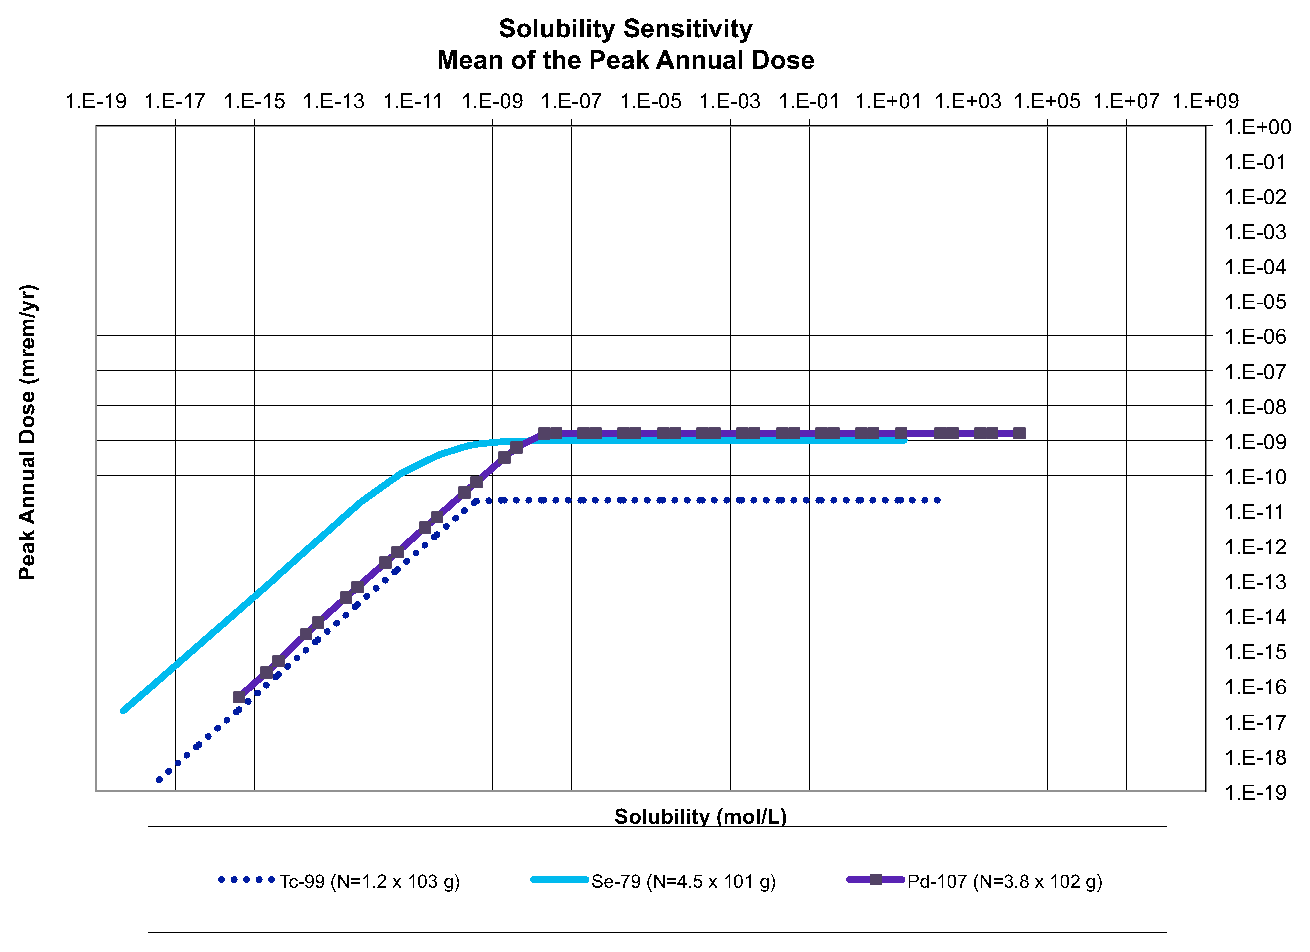
\includegraphics[width=0.7\linewidth]{./nuclide_demonstration/Solubility_Summary_Sol.eps}
\caption{Solubility limit sensitivity. The peak annual dose due to an inventory, 
$N$, of each isotope.}
\label{fig:SolSum}
\end{figure}
\end{frame}


\begin{frame}[ctb!]
\frametitle{Cyder Solubility Sensitivity}
In the parametric analysis of \Cyder performance, it was shown that the 
solubility sensitivity behavior closely matched that of the GDSM 
sensitivity behaviors. In agreement with expectations, \Cyder results in Figure 
\ref{fig:sol_result}, demonstrate a sharp turnover 
where the solubility limit exceeds the point at which it limits movement. 

\begin{figure}[htbp!]
\begin{center}
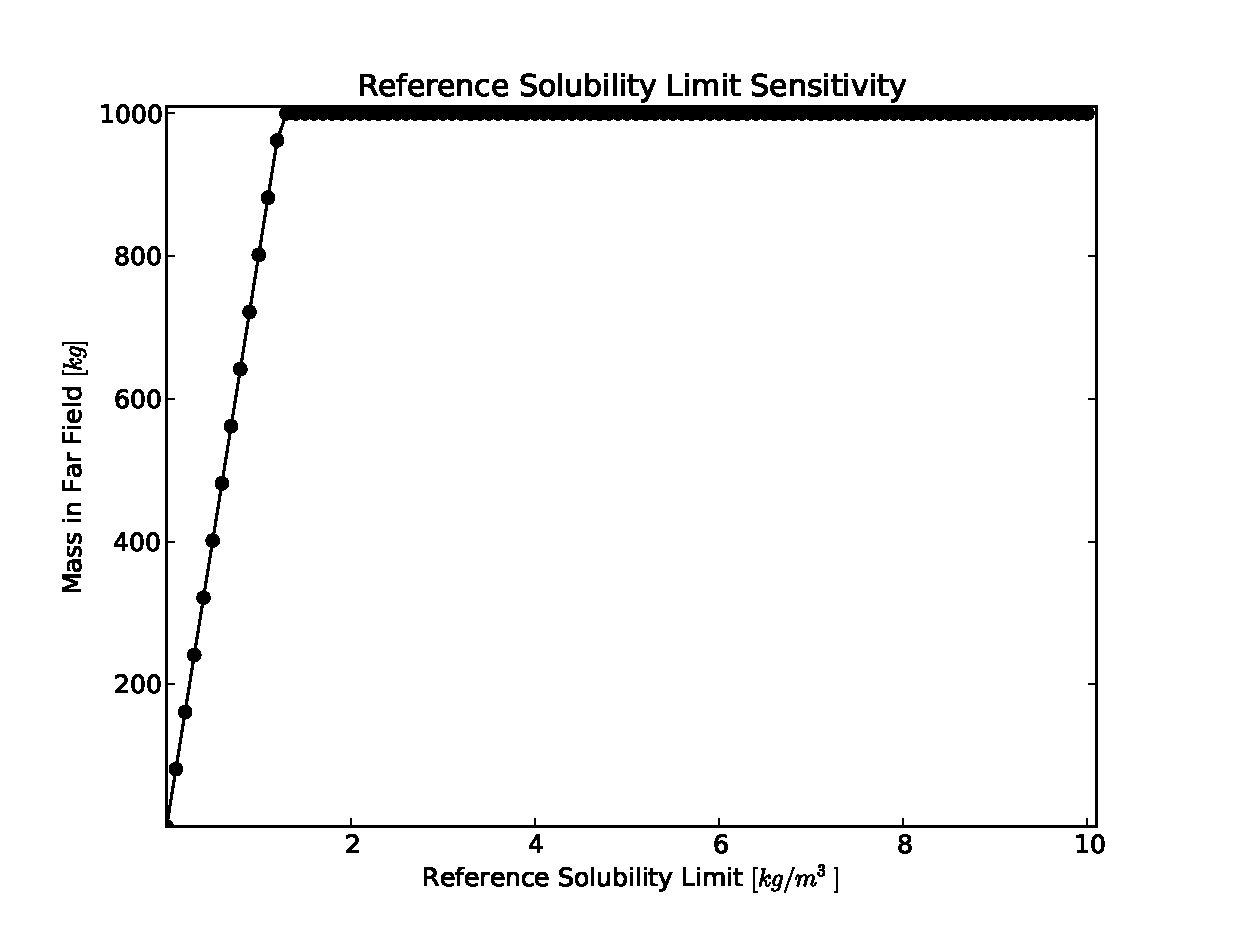
\includegraphics[width=0.7\linewidth]{./nuclide_demonstration/sol.eps}
\end{center}
\caption{Sensitivity demonstration of solubility limitation in \Cyder for an 
arbitrary isotope assigned a variable solubility limit. }
\label{fig:sol_result}
\end{figure}

\end{frame}


